\secnumbersection{MARCO CONCEPTUAL}

\subsection{\textit{Qubits}, compuertas y algoritmos cuánticos}

Un \textit{qubit} puede ser entendido desde la perspectiva de un sistema físico que tiene un comportamiento de sistema de dos niveles (entre otras muchas características), pero también se puede entender desde una perspectiva más matemática. Para esta memoria, se tomará esta segunda perspectiva (debido a que se buscan aplicaciones de alto nivel), para ello se parte de la premisa de que no importa de que está hecho el \textit{qubit}, sino que, nos importa la descripción y las propiedades matemáticas asociadas a este objeto.

\subsubsection{Que es un \textit{qubit}}
Un \textit{qubit} al igual que un bit, corresponde a un estado, pero a diferencia de este último (que solo puede estar en $0$ o $1$), los \textit{qubits} pueden estar en una infinidad de estados gracias a la combinación lineal de los estados basales. 
\begin{equation*}
    \ket{\psi} = \alpha \ket{0} + \beta \ket{1}
\end{equation*}
Donde $\alpha$ y $\beta$ corresponden a números complejos que cumplen con $|\alpha|^2 + |\beta|^2 = 1$. Esto es posible, ya que, los \textit{qubits} son objetos que se rigen por las leyes de la mecánica cuántica, las cuales permiten construir estados como combinaciones lineales mientras estos no sean observados, en el momento de que esto ocurra el estado colapsa a uno de los que componen la combinación lineal y este objeto cuántico pasa a comportarse como uno clásico. En la literatura, es común encontrar a los \textit{qubits} representados como esferas \ref{fig:EsferaBloch}, siendo los estados, puntos del manto de la misma. Esta representación se conoce como la esfera de Bloch.

\begin{figure}[H]
\centering
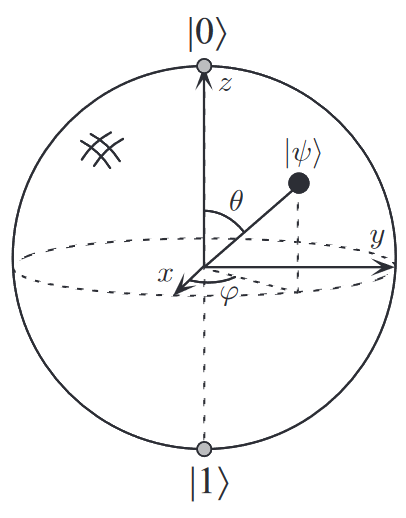
\includegraphics[width=0.3\textwidth]{figures/S2/ESFERABLOCH.png}
\caption{\label{fig:EsferaBloch} Representación de un \textit{qubit} en la esfera de Bloch. Fuente: \cite{nielsen_chuang_2010}}
\end{figure}

Para construir un estado de un sistema de muchos \textit{qubits} (independientes entre sí), lo que se realiza es aplicar el producto Kronecker (producto tensorial) entre cada uno de los estados, lo que crea un vector de tamaño $2^n$ (siendo $n$ el número de \textit{qubits}). La notación de este producto es equivalente a la de muchos bits $\ket{\psi_1\psi_2 ... \psi_n}$ (los $\psi_i$ corresponde a los estados de cada \textit{qubit}).

\subsubsection{Como operar con un \textit{qubit}}
Las acciones que se aplican a los \textit{qubits} corresponden a la aplicación de operadores, estos operadores en la literatura son conocidos como compuertas. Una de las ideas claves es el concepto de la reversibilidad de las operaciones, es decir, que después de aplicar una cierta secuencia de operaciones a un estado inicial, podamos ser capaces de volver al estado original, para lograr esto, se pide que las compuertas sean unitarias, esto quiere decir que, siendo $U$ una compuerta, tiene que verificar $UU^{\dag}=U^{\dag}U=I$.

En la literatura, es común que las compuertas sean presentadas en dos grupos, las compuertas de un solo \textit{qubit} y las de muchos \textit{qubits}. Las compuertas de un solo \textit{qubit} se interpretan como operadores de rotación (teniendo en mente la esfera de Bloch), lo que hacen estos operadores es mover el estado por el manto de la esfera. A continuación, se entrega la descripción matricial junto a una interpretación rotacional de las matrices de un solo \textit{qubits} más famosas.

\begin{enumerate}
 \item Compuerta X: Esta compuerta lo que realiza es un intercambio entre la probabilidad de los estados, es decir, aplica una rotación de 180 grados respecto al eje X.
    \begin{equation*}
    X = 
        \begin{pmatrix}
        0 & 1\\
        1 & 0
        \end{pmatrix}
    \end{equation*} 
    \item Compuerta Y: Puede ser entendida como una rotación respecto al eje Y por 180 grados.
    \begin{equation*}
    Y = 
        \begin{pmatrix}
        0 & -i\\
        i & 0
        \end{pmatrix}
    \end{equation*} 
    \item Compuerta Z: Esta compuerta realiza un cambio de signo de la componente $\ket{1}$. Al igual que las compuertas anteriores, también es una rotación respecto al eje Z por 180 grados.
    \begin{equation*}
    Z = 
        \begin{pmatrix}
        1 & 0\\
        0 & -1
        \end{pmatrix}
    \end{equation*}
    \item Compuerta I: La compuerta identidad no realiza nada, deja el \textit{qubit} en el mismo estado.
    \begin{equation*}
    I = 
        \begin{pmatrix}
        1 & 0\\
        0 & 1
        \end{pmatrix}
    \end{equation*} 
    \item Compuerta Hadamard: Esta compuerta también es conocida como la compuerta de superposición, ya que la acción que realiza es llevar un estado cualquiera a un estado de superposición entre los vectores de la base. Esto puede ser entendido como una rotación de 180 grados respecto a los ejes Z y X.
    \begin{equation*}
    H = \frac{1}{\sqrt{2}}
        \begin{pmatrix}
        1 & 1\\
        1 & -1
        \end{pmatrix}
    \end{equation*} 
    \item Compuerta de fase: Esta compuerta está conectada con la compuerta Z por $S^2 = Z$, donde, al igual que esta, realiza una rotación de 90 grados respecto al eje Z
    \begin{equation*}
    S = 
        \begin{pmatrix}
        1 & 0\\
        0 & i
        \end{pmatrix}
    \end{equation*} 
    \item Compuerta pi octavos: Al igual que la compuerta de fase, esta también tiene una relación con la compuerta Z, $T^2=S$ por lo tanto $T^4=Z$, tomando esta relación, es que esta compuerta se entiende como una rotación de 45 grados respecto al eje Z
    \begin{equation*}
    T = 
        \begin{pmatrix}
        1 & 0\\
        0 & exp(\frac{i\pi}{4})
        \end{pmatrix}
    \end{equation*} 
    \item Compuerta de rotación: Como su nombre lo indica, es un conjunto de compuertas cuya función es rotar el estado actual en función de un eje (indicado como subíndice) por $\theta$ grados.
   \begin{align*}
    R_x(\theta) &=
    \begin{pmatrix}
    cos(\frac{\theta}{2}) & -isen(\frac{\theta}{2})\\
    -isen(\frac{\theta}{2}) & cos(\frac{\theta}{2})
    \end{pmatrix} \\
    R_y(\theta) &=
    \begin{pmatrix}
    cos(\frac{\theta}{2}) & -sen(\frac{\theta}{2})\\
    -sen(\frac{\theta}{2}) & cos(\frac{\theta}{2})
    \end{pmatrix} \\
    R_z(\theta) &=
    \begin{pmatrix}
    exp(-i\frac{\theta}{2}) & 0\\
    0 & exp(i\frac{\theta}{2})
    \end{pmatrix}
    \end{align*}
    \item Compuerta de medición: Esta compuerta indica la medición del \textit{qubit}, es decir, sé ''observa'' el \textit{qubit} y se obtiene una proyección sobre uno de los estados basales que componen al vector de estado en ese momento del circuito. No posee una representación matricial, es más una representación de ensamble donde se almacenan todos los estados basales con la probabilidad de aparición.
\end{enumerate}

Las primeras cuatro compuertas son conocidas como matrices de Pauli (también se denotan como $\sigma^{X}$, $\sigma^{Y}$, $\sigma^{Z}$, $\sigma^{I}$ respectivamente) y nos serán útil en varias descripciones de los capítulos siguientes. 

Pasando a las compuertas de muchos \textit{qubits}, a diferencia de las anteriores, su objetivo es romper con la independencia de los estados, creando correlaciones entre los mismos. A continuación, se muestra la representación por bloques junto a una breve descripción de las compuertas más famosas.


\begin{enumerate}
    \item Compuerta control X: Esta compuerta es una compuerta condicional de dos \textit{qubit}, que solo se activa en caso de encontrar $\ket{1}$ en el \textit{qubit} de control, en tal caso, aplica la compuerta $X$ en el \textit{qubit} de \textit{target}. Esta compuerta también es conocida como CNOT.
    \begin{equation*}
    CX = 
        \begin{pmatrix}
        I & 0\\
        0 & X
        \end{pmatrix}
    \end{equation*} 
    \item Compuerta control: Corresponden a una versión generalizada de la compuerta CNOT donde la compuerta X es reemplazada por una compuerta cualquiera, cumpliendo la misma función (aplicar la compuerta en caso de tener $\ket{1}$).
    \begin{equation*}
    CU = 
        \begin{pmatrix}
        I & 0\\
        0 & U
        \end{pmatrix}
    \end{equation*} 
\end{enumerate}


\subsubsection{Circuitos y algoritmos cuánticos}
Ahora que tenemos los elementos básicos, podemos pasar a hablar sobre los circuitos cuánticos y como se utilizan para desarrollar algoritmos. Antes de ello, se presentará la notación de las compuertas y circuitos.

\begin{figure}[H]
\centering
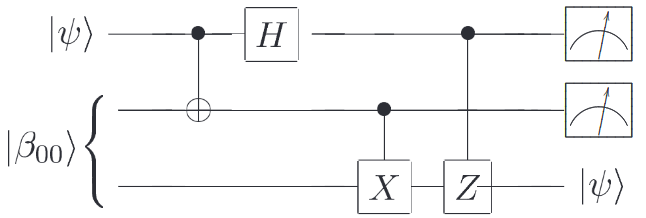
\includegraphics[width=0.6\textwidth]{figures/S2/EJEMPLOCIRCUITO.png}
\caption{\label{fig:CircuitExample} Ejemplo de circuito cuántico. Fuente: \cite{nielsen_chuang_2010}}
\end{figure}

Un circuito cuántico no es otra cosa que un conjunto de \textit{qubits} a los cuales se les aplican compuertas de manera secuencial, ver imagen \ref{fig:CircuitExample}. Los \textit{qubits} son representados como líneas horizontales, dotándoles así de una secuencialidad a la hora de aplicarles compuertas. Al tener varios \textit{qubits}, estos se representan como líneas horizontales paralelas. Usando la notación visual de las compuertas, ver figura \ref{fig:GatesGraphical}, las compuertas son colocadas encima de las líneas, indicando así que esta fue aplicada a ese \textit{qubit}.

Un detalle importante es que si bien los \textit{qubits} son representados de forma paralela, esto no es necesariamente la topología real que tienen, por ejemplo, cuando se simularan los \textit{qubits}, estos tienen conexiones para todos los otros, esto en representación de grafos corresponde a un grafo completo, en el caso de máquinas reales, no todos los \textit{qubits} se pueden conectar con todos (va a estar delimitado por el \textit{hardware}).

\begin{figure}[H]
\centering
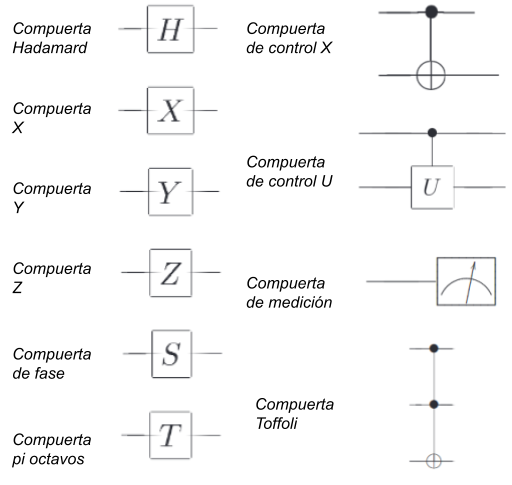
\includegraphics[width=0.7\textwidth]{figures/S2/COMPUERTASVISUAL.png}
\caption{\label{fig:GatesGraphical} Notación gráfica de las compuertas cuánticas. Fuente: \cite{nielsen_chuang_2010}}
\end{figure}

Finalmente, un algoritmo cuántico no es otra cosa que un circuito cuántico cuyas compuertas son elegidas con el objetivo de maximizar las probabilidades de un conjunto de estados que corresponden a la solución del problema. Un tipo famoso de algoritmos en la época NISQ son los algoritmos híbridos, estos son algoritmos con una parte cuántica y una parte clásica, la parte cuántica suele corresponder a la construcción y ejecución de un \textit{ansatz} (término que se explicara más adelante, pero entiéndase como una matriz con parámetros) y la parte clásica es la resolución de un problema de minimización de los parámetros del \textit{ansatz} utilizando algún algoritmo clásico de optimización.

%
%
%
%
%


\newpage
\subsection{Principios básicos y campos de investigación de la materia en estado sólido} 

Esta sección no es una introducción ni a la materia condensada ni a la termodinámica ni a la química cuántica, se asumirá que el lector tiene conocimientos básicos de mecánica cuántica, termodinámica y química. La idea es solo presentar conceptos claves para el desarrollo de la memoria.


\subsubsection{Un poco de química}

Antes de pasar a hablar de como interactúan muchos átomos, es necesario partir hablando de solo uno. La pregunta que surge naturalmente es ¿Qué es un átomo?, un átomo se encuentra compuesto por electrones, protones y neutrones que interactúan entre sí, entonces, nuestros elementos bases para estudiar la materia y su comportamiento van a ser los electrones, protones y neutrones.


Lo primero que hay que revisar es el cómo se construyen los átomos. A la fecha, en la tabla periódica se informan 120 elementos, que difieren en el número atómico, como cada átomo tiene un número diferente de electrones, entonces, la pregunta es ¿cómo se distribuyen estos electrones para formar el átomo?, para ello, debemos introducir el concepto de estructura electrónica de los átomos. 

Como bien se sabe, los electrones en un átomo tienen cuatro números cuánticos ($n$, $l$, $m_l$ y $m_s$), los primeros tres describen la región en donde es más probable encontrar al electrón y el último indica la orientación de su espín. Los electrones son agrupados dentro de capas que están determinadas por el núcleo del átomo, cuanto más grande sea, mayor será el número de capas (por lo tanto, mayor número de electrones). Cada capa tiene un número de subcapas, las cuales contienen un conjunto finito de orbitales. Un orbital no es otra cosa que una región dentro de un átomo en donde un electrón puede ser encontrado, cada orbital puede contener un número finito de electrones.

Cada orbital tiene un número de sitios que pueden ser ocupados por los electrones, el orbital $s$ tiene un sitio, él $d$ tiene tres sitios, él $p$ tiene 5 sitios y él $f$ tiene 14 sitios. Cada sitio puede contener dos electrones, los cuales, por el principio de exclusión de Pauli, deben tener un número cuántico $m_s$ distinto.

Con lo anterior expuesto, podemos pasar a hablar de la estructura electrónica, la cual, no es otra cosa que un arreglo de los electrones sobre las distintas capas. Para ello presentaremos las reglas de Hund y el principio de Aufbau.

El principio de Aufbau fue formulado por Niels Bohr y Wolfgang Pauli en el año 1920, en él se indica que para que los electrones ocupen orbitales de mayor energía deben ocupar por completo los orbitales de menor energía. Por ejemplo, para que los electrones ocupen un orbital $p$, deben ocupar todos los orbitales $s$. Por otro lado, las reglas de Hund son un conjunto de postulados derivados de forma empírica, estos fueron presentados alrededor del 1927 por Friedrich Hund. Las reglas son las siguientes
\begin{enumerate}
    \item El estado de mínima energía es aquel con la mayor multiplicidad del espín.
    \item Para términos con la misma multiplicidad del espín, aquel con el orbital de mayor momento angular, será él con menor energía.
\end{enumerate}

\subsubsection{Modelos sobre el comportamiento de los átomos}
Lo siguiente que tenemos que revisar es el cómo se modelan estas interacciones entre las partículas que componen a los átomos. La expresión general\cite{szabo1996modern} tiene en cuenta todas las posibles interacciones, las cuales se reflejan en las distintas sumatorias de la expresión.

\begin{equation*}
    \mathcal{H} = -\sum_{i=!}^{N}\frac{1}{2}\nabla_i^2 - \sum_{A = 1}^{M} \frac{1}{2M_A}\nabla_A^{2} -\sum_{i=1}^{N}\sum_{A = 1}^{M} \frac{Z_A}{r_{iA}} + \sum_{i=1}^{N}\sum_{j>i}^{N} \frac{1}{r_{ij}}  + \sum_{A=1}^{M}\sum_{B>A}^{M} \frac{Z_AZ_B}{R_{AB}}
\end{equation*}

El problema de esta expresión es el número de grados de libertad y de interacciones que considera, en estructuras complejas es computacionalmente inviable trabajar directamente con esta expresión. Frente a este problema, se han propuesto diferentes aproximaciones que se concentran en modelar características concretas de la materia, lo cual permite reducir la cantidad de grados de libertad (además de considerar ciertos supuestos sobre las interacciones). Una de las aproximaciones más famosa es la de Born-Oppenheimer\cite{BornOppenheimer} donde la idea es que como las partículas del núcleo son más pesadas que los electrones, entonces su velocidad es comparablemente menor que la de los electrones, entonces los términos de la energía cinética y la energía de repulsión (este término se vuelve constante) del núcleo pueden ser despreciados (este se conoce como hamiltoniano electrónico). De esta forma, la expresión anterior se reduce a la siguiente
\begin{equation*}
    \mathcal{H}_{elec} = -\sum_{i=!}^{N}\frac{1}{2}\nabla_i^2  -\sum_{i=1}^{N}\sum_{A = 1}^{M} \frac{Z_A}{r_{iA}} + \sum_{i=1}^{N}\sum_{j>i}^{N} \frac{1}{r_{ij}}
\end{equation*}

De este tipo de aproximaciones es que surgieron diferentes tipos de hamiltonianos que buscan modelar interacciones concretas. acá solo expondremos un par de hamiltonianos. El primer corresponde al hamiltoniano electrónico (también conocido como hamiltoniano de Coulomb) antes mostrado, pero en su forma de segunda cuantización\cite{szabo1996modern}:
\begin{equation}
    \mathcal{H} = \sum_{pq} h_{pq} a^{\dag}_{p} a_{q}  + \frac{1}{2} \sum_{pqrs}h_{pqrs} a^{\dag}_{p}a^{\dag}_{q} a_{r}a_{s}
    \label{eq:SCmolecular}
\end{equation}
Las constantes que acompañan a cada término se definen como las siguientes integrales $h_{pq} = \int \phi^{*}_p(r)(-\frac{1}{2} \nabla^{2} - \sum_I \frac{Z_I}{R_I-r})\phi_q(r) dr$ y $h_{pqrs} = \int \frac{\phi^{*}_p(r_1) \phi^{*}_q(r_2) \phi_r(r_2) \phi_s(r_1) }{|r_1 -r_2|} dr_1 dr_2$.


El siguiente modelo es el Modelo de Heisenberg\cite{Heisenberg1928}, este fue propuesto por Werner Heisenberg para estudiar los cambios de fase y puntos críticos de materiales magnéticos. La expresión matemática del modelo es la siguiente:
\begin{equation}
    \mathcal{H} = \sum_{\<i,j\>} -J \cdot S_i\cdot S_j = \sum_{\<i,j\>} -J^x_{ij}(\sigma^x_i\sigma^x_j) -J^y_{ij}(\sigma^y_i\sigma^y_j) -J^z_{ij}(\sigma^z_i\sigma^z_j)
    \label{eq:Heisenberg}
\end{equation}
En este caso, los espines son modelados usando las matrices de Pauli correspondientes al espín. Este modelo, a pesar de su simpleza, describe bien el comportamiento de sistemas sintetizados y que se encuentran en la naturaleza, además es utilizado para el estudio de transiciones de fase cuántica, superconductividad, entre otras\cite{IntroHeisenberg}. 

Finalmente, el último modelo es el modelo de Hubbard\cite{HubbardModel}. John Hubbard propuso este modelo para modelar el efecto de las correlaciones en las bandas de energía. A continuación, se muestra la ecuación del modelo de Hubbard utilizando operadores de segunda cuantización.
\begin{equation}
    \mathcal{H} = -t \sum_{\expval{i,j}, \sigma}( a^{\dag}_{i, \sigma} a_{j, \sigma} + h.c) + U\sum_{j}n_{j\uparrow}n_{j\downarrow}
    \label{eq:FHHamiltonian}
\end{equation}
El término $t$ corresponde a la energía cinética de los electrones, mientras que el término $U$ corresponde a la interacción efectiva. Una de las motivaciones por estudiar este modelo, es que a pesar de su simpleza, captura bien los fenómenos cuánticos de sistemas con parámetros de características más generales\cite{HubbardModelBook}. Un detalle importante es que con $U = 0$ se obtiene el modelo de \textit{tight-binding}, así que, por comodidad, ambos modelos serán considerados como el mismo.


Todos estos modelos están expresados en su forma más elemental, se le pueden agregar más interacciones para hacer de estos algo más completo y realista, pero, todo esto dependerá de lo que se quiere estudiar.


\subsubsection{Mediciones}

El siguiente tema por tratar es el cómo extraer información útil de los sistemas, existen muchas técnicas experimentales que permiten cuantificar características del sistema, como la espectroscopia, la fluorescencia, entre otros. El problema con esto es que esas técnicas pertenecen al dominio de la física experimental, para efectos de esta memoria, nos concentraremos en las descripciones matemáticas de ciertas cantidades, conocidas en la literatura como observables, las cuales pueden ser calculadas numéricamente teniendo el hamiltoniano. En esta sección presentaremos algunas de las más relevantes y utilizadas en la literatura, para ello tengamos en mente que tenemos un hamiltoniano arbitrario $\mathcal{H}$.

El valor esperado de un operador $O$ con consideración de la temperatura se define como:
\begin{equation*}
    \expval{O} = Tr[\rho O] = \frac{1}{Z}\sum_i \exp{\frac{-E_i}{k_bT}}\bra{\psi_i}O\ket{\psi_i}
\end{equation*}
Donde $\rho = \frac{1}{Z}\sum_i \exp{\frac{-E_i}{k_bT}}\ket{\psi_i}\bra{\psi_i}$. Independiente de la expresión, se requiere tener de forma obligatoria los $E_i$ y $\ket{\psi_i}$ que corresponden a los valores y vectores propios del hamiltoniano, por otro lado, el término $Z$ corresponde a función de partición que se define como $Z = \sum_i \exp{\frac{-E_i}{k_bT}}$ (la cual permite normalizar las exponenciales) y por último, $k_b$ que corresponde a la constante de Boltzmann.

Un caso particular es cuando $T=0$, y es un punto donde solo los estados de mínima energía pueden sobrevivir (los otros estados tienen probabilidades nulas). De igual forma, uno, puede calcular valores esperados usando un solo estado, por ejemplo, el de mínima energía bajo el supuesto de trabajar a temperatura 0 o un estado que evoluciona respecto al tiempo. Matemáticamente, esto se define como:

\begin{equation*}
    \expval{O} = \bra{\psi} O \ket{\psi}
\end{equation*}

Existe una gran cantidad de observables\cite{EfectoMagnetocalorico}, pero para esta memoria nos enfocaremos en dos observables, la magnetización y el calor especifico. La magnetización suele estudiarse en sistemas de espines y se busca caracterizar la orientación de estos, en ese caso se considera una magnetización parcial, ya que nos concentramos en un subconjunto.
\begin{equation*}
    \expval{M} = \sum_i \expval{m_i} = \sum_i \frac{1}{Z}(\sum_j \exp{\frac{-E_j}{Tk_b}} \bra{E_j}m_i\ket{E_j})
\end{equation*}
Los términos $m_i$ corresponden a la magnetización en cada sitio, de forma individual. Por otro lado, el calor específico se define como la cantidad de energía necesaria para elevar la temperatura de un material en una unidad, matemáticamente se define de la siguiente forma:
\begin{equation*}
    c_b = \frac{\expval{\mathcal{H}^2}- \expval{\mathcal{H}}^2}{T^2k_b}
\end{equation*}

Un detalle que es necesario aclarar es hay que tener cuidado a la hora de calcular un observable a un hamiltoniano, ya que, se debe tener en cuenta que el observable tiene sentido en este.

\subsection{Codificación y trabajo en el espacio de espines}

\subsubsection{Codificación de Jordan Wigner}
Esta es una de las codificaciones más intuitivas que permiten conectar operadores de segunda cuantización con operadores de espines. La idea es utilizar que las matrices de Pauli conforman una base del espacio de matrices de $2x2$, por lo tanto, es posible generar una descomposición en esta base de los diferentes operadores. Dicho esto, a continuación se mostrarán equivalencias de los operadores de creación y aniquilación respectivamente (las operaciones omitidas son los productos Kronecker) \cite{Lana}:
\begin{equation*}
    a_j^{\dag} = \sigma_0^Z \cdots \sigma^Z_{j-1} \frac{1}{2}(\sigma^X_j -i\sigma^Y_j) \sigma^I_{j+1} \cdots \sigma^I_{n} 
\end{equation*}
\begin{equation*}
    a_j = \sigma^Z_0 \cdots \sigma^Z_{j-1}  \frac{1}{2}(\sigma^X_j +i\sigma^Y_j) \sigma^I_{j+1} \cdots \sigma^I_{n}
\end{equation*}
Con estas dos equivalencias, es posible derivar las representaciones en el espacio de espines de los otros operadores (como el número de partículas entre otros). Una de las características más relevantes de esta nueva representación, es que todos los operadores de segunda cuantización pueden ser expresados como un producto tensorial de sistemas aislados. 

Dentro de la literatura existen otras codificaciones más eficientes, respecto al número de \textit{qubits} necesarios, como la de Bravyi-Kitaev y de paridad \cite{JW-BK-COD}.

\subsubsection{Ejemplo de representación de hamiltonianos}

Para ejemplificar el cómo utilizar esta transformación, tomaremos el hamiltoniano en segunda cuantización para el dímero de hidrógeno (distancia de $0.775$ (ángstrom) y basis set ''sto-3g''), el cual se resume en la siguiente expresión:

\begin{multline*}
     \mathcal{H} = -1.25633( a_0^{\dag} a_0 ) + -0.47189( a_1^{\dag} a_1 ) + -1.25633( a_2^{\dag} a_2 ) + -0.47189( a_3^{\dag} a_3 ) \\
+ 0.33785( a_0^{\dag}a_0^{\dag} a_0 a_0 ) + 0.09046( a_0^{\dag} a_0^{\dag} a_1 a_1 ) + 0.09046( a_0^{\dag} a_1^{\dag} a_0 a_1 ) + 0.33229( a_0^{\dag} a_1^{\dag} a_1 a_0 ) \\
+ 0.33785( a_0^{\dag} a_2^{\dag} a_2 a_0 ) + 0.09046( a_0^{\dag} a_2^{\dag} a_3 a_1 ) + 0.09046( a_0^{\dag} a_3^{\dag} a_2 a_1 ) + 0.33229( a_0^{\dag} a_3^{\dag} a_3 a_0 ) \\
+ 0.33229( a_1^{\dag} a_0^{\dag} a_0 a_1 ) + 0.09046( a_1^{\dag} a_0^{\dag} a_1 a_0 ) + 0.09046( a_1^{\dag} a_1^{\dag} a_0 a_0 ) + 0.34928( a_1^{\dag} a_1^{\dag} a_1 a_1 ) \\
+ 0.33229( a_1^{\dag} a_2^{\dag} a_2 a_1 ) + 0.09046( a_1^{\dag} a_2^{\dag} a_3 a_0 ) + 0.09046( a_1^{\dag} a_3^{\dag} a_2 a_0 ) + 0.34928( a_1^{\dag} a_3^{\dag} a_3 a_1 ) \\
+ 0.33785( a_2^{\dag} a_0^{\dag} a_0 a_2 ) + 0.09046( a_2^{\dag} a_0^{\dag} a_1 a_3 ) + 0.09046( a_2^{\dag} a_1^{\dag} a_0 a_3 ) + 0.33229( a_2^{\dag} a_1^{\dag} a_1 a_2 ) \\
+ 0.33785( a_2^{\dag} a_2^{\dag} a_2 a_2 ) + 0.09046( a_2^{\dag} a_2^{\dag} a_3 a_3 ) + 0.09046( a_2^{\dag} a_3^{\dag} a_2 a_3 ) + 0.33229( a_2^{\dag} a_3^{\dag} a_3 a_2 ) \\
+ 0.33229( a_3^{\dag} a_0^{\dag} a_0 a_3 ) + 0.09046( a_3^{\dag} a_0^{\dag} a_1 a_2 ) + 0.09046( a_3^{\dag} a_1^{\dag} a_0 a_2 ) + 0.34928( a_3^{\dag} a_1^{\dag} a_1 a_3 ) \\
+ 0.33229( a_3^{\dag} a_2^{\dag} a_2 a_3 ) + 0.09046( a_3^{\dag} a_2^{\dag} a_3 a_2 ) + 0.09046( a_3^{\dag} a_3^{\dag} a_2 a_2 ) + 0.34928( a_3^{\dag} a_3^{\dag} a_3 a_3 ) 
\end{multline*}

Tomando el término $a_0^{\dag} a_0$. Si aplicamos la transformación de Jordan-Wigner considerando $n=4$, tenemos el siguiente producto:

\begin{equation*}
    a_0^{\dag} a_0 = (\frac{1}{2}(\sigma^X_0 -i\sigma^Y_0)\otimes\sigma^I_1\otimes\sigma^I_2\otimes\sigma^I_3) (\frac{1}{2}(\sigma^X_0 +i\sigma^Y_0)\otimes\sigma^I_1\otimes\sigma^I_2\otimes\sigma^I_3)
\end{equation*}

Como solo el primer sitio tiene operadores distintos a la identidad, podemos desarrollar el producto, llegando a $(\sigma^X_0 -i\sigma^Y_0)(\sigma^X_0 +i\sigma^Y_0) = 2\sigma_0^I + i\sigma_0^X\sigma_0^Y - i\sigma_0^Y\sigma_0^X$. Entonces, el término original es representado en el espacio de espines como (se omitirán los productos tensoriales):

\begin{equation*}
    a_0^{\dag} a_0 = \frac{1}{2}\sigma^I_0\sigma^I_1\sigma^I_2\sigma^I_3 + \frac{i}{4}(\sigma^X_0\sigma^Y_0)\sigma^I_1\sigma^I_2\sigma^I_3 - \frac{i}{4}(\sigma^Y_0\sigma^X_0)\sigma^I_1\sigma^I_2\sigma^I_3
\end{equation*}


Siguiendo este procedimiento con el resto de los términos, podemos reescribir el hamiltoniano de segunda cuantización en el espacio de espines, el cual es mostrado a continuación:

\begin{multline*}
\mathcal{H} = -0.81054\sigma_0^I\sigma_1^I\sigma_2^I\sigma_3^I + 0.17218\sigma_0^I\sigma_1^I\sigma_2^I\sigma_3^Z - 0.22575\sigma_0^I\sigma_1^I\sigma_2^Z\sigma_3^I \\
+ 0.17218\sigma_0^I\sigma_1^Z\sigma_2^I\sigma_3^I - 0.22575\sigma_0^Z\sigma_1^I\sigma_2^I\sigma_3^I + 0.12091\sigma_0^I\sigma_1^I\sigma_2^Z\sigma_3^Z \\
+ 0.16892\sigma_0^I\sigma_1^Z\sigma_2^I\sigma_3^Z + 0.04523\sigma_0^Y\sigma_1^Y\sigma_2^Y\sigma_3^Y + 0.04523\sigma_0^X\sigma_1^X\sigma_2^Y\sigma_3^Y \\
+ 0.04523\sigma_0^Y\sigma_1^Y\sigma_2^X\sigma_3^X + 0.04523\sigma_0^X\sigma_1^X\sigma_2^X\sigma_3^X + 0.16614\sigma_0^Z\sigma_1^I\sigma_2^I\sigma_3^Z \\
+ 0.16614\sigma_0^I\sigma_1^Z\sigma_2^Z\sigma_3^I + 0.17464\sigma_0^Z\sigma_1^I\sigma_2^Z\sigma_3^I + 0.12091\sigma_0^Z\sigma_1^Z\sigma_2^I\sigma_3^I
\end{multline*}

Ambos hamiltonianos son equivalentes y reflejan la misma física del sistema. Lo importante de esta transformación es que el segundo hamiltoniano es más fácil de construir y trabajar en computador, ya que, que los operadores de espines tienen descripciones matriciales directas a diferencia de los operadores de segunda cuantización.


%
%
%
%
%
\subsection{Como utilizar los ordenadores cuánticos para hacer física}
En esta sección, se presentarán los componentes básicos para poder extraer física de los cálculos realizados dentro de los circuitos cuánticos.

\subsubsection{\textit{Ansatz}}
Uno puede definirse un estado arbitrario con el cual partir el circuito, pero para poder conectarlo con el problema, es necesario que exista una serie de compuertas que permitan ir variando este estado inicial y que se ajuste a lo que buscamos. Esta descripción se conoce normalmente como \textit{ansatz}, estos suelen estar parametrizados por un vector $\theta$, donde las componentes son valores que permiten ir ajustando la rotación derivada de las compuertas del \textit{ansatz} ($\ket{\psi(\theta)} = U(\theta)\ket{\psi_0}$). De esta forma, es posible ir ajustando los parámetros para que nuestro vector inicial se ajuste al problema que intentamos solucionar. 

Los \textit{ansatz} son altamente utilizados en los algoritmos variacionales cuánticos, ya que, el \textit{ansatz} puede ser simulado de forma eficiente en un ordenador cuántico. Una de las limitaciones de los \textit{anzats}, es que, como son responsables de generar el espacio de posibles estados, una elección incorrecta del mismo puede derivar en soluciones sin sentido. A continuación, se mostrarán los \textit{ansatz} más utilizados en la literatura.

El \textit{hardware efficient ansatz}\cite{EfficientAnsatz} corresponde a uno de los tipos de \textit{ansatz} más generales y fue diseñado para ser implementado en dispositivos NISQ. La idea es descomponer un operador unitario local genérico como el producto de las compuertas de rotación $R_x, R_y$ y $R_z$, uno de los problemas de esto es el crecimiento del número de parámetros necesario, ya que, por cada compuerta se requieren $3$ parámetros, lo cual, para $n$ \textit{qubits} y una profundidad $D$ se requieren $3nD$ \textit{qubits}.
\begin{equation*}
    U(\theta) = \prod_{d=1}^{D} U_{ent} \prod_{i=1}^{n} R_z(\theta_1^{i,d})R_x(\theta_2^{i,d})R_y(\theta_3^{i,d})
\end{equation*}
Este \textit{ansatz} tiene un buen rendimiento para un bajo número de \textit{qubits} (2-6), pero presenta un problema de desvanecimiento del gradiente a medida que se aumenta el número de \textit{qubits}, en ratio de decrecimiento es de tipo exponencial\cite{DesvanecimientoGradiente}. 

El \textit{unitary coupled cluster} (UCC)\cite{doi:10.1021/acs.jctc.8b01004}\cite{Fedorov2022} es utilizando en el contexto de química cuántica y materia condensada. A diferencia del \textit{ansatz} anterior, en este sí incluye contexto del problema, considerando los orbitales de las moléculas. El \textit{coupled cluster} tradicional se define de la siguiente manera
\begin{equation*}
    \hat{T} = \hat{T_1} + \hat{T_2} = \sum_{i,a} t_i^a \hat{a_a}^{\dag} \hat{a_i} + \frac{1}{4}\sum_{i,j,a,b} t_{ij}^{ab} \hat{a_a}^{\dag} \hat{a_b}^{\dag} \hat{a_j}\hat{a_i}
\end{equation*}
Este puede tener más términos, pero para efectos practicas con dos son suficientes. Lamentablemente, al aplicarle la exponencial a $\hat{T}$, lo que se obtiene no es un operador unitario, por lo tanto, no puede ser representado como un circuito. Por lo tanto, para definir el \textit{ansatz} se define de la siguiente forma:
\begin{equation*}
    U = exp(\hat{T} - \hat{T}^{\dag})
\end{equation*}
Este se conoce como \textit{Unitary Coupled Cluster Single Doubles} (UCCSD), luego tenemos otra variante llamada \textit{k-Unitary pair Coupled Cluster Generalized Singles and Doubles Product Wavefunctions} (k-UpCCGSD), la cual se define de mediante la siguiente productoria:
\begin{equation*}
    U = \prod_{\alpha=1}^{k} exp(\hat{T^{\alpha}} - \hat{T^{\alpha}}^{\dag}) 
\end{equation*}
La diferencia respecto al anterior sobre el término $\hat{T_2}$, el cual se define de la siguiente forma:
\begin{equation*}
    \hat{T_2} = \sum_{i,\alpha} t_{i_{\alpha} i_{\beta}}^{a_{\alpha} a_{\beta}} \hat{a}^{\dag}_{a_{\alpha}} \hat{a}^{\dag}_{a_{\beta}} \hat{a}_{i_{\beta}} \hat{a}_{i_{\alpha}}
\end{equation*}

Ambos, como su nombre indican, solo consideran interacciones individuales y entre pares, es posible extender estos \textit{ansatz} para que consideren más interacciones, lo cual no es otra cosa que agregar más términos $\hat{T_i}$.

El \textit{variational hamiltonian ansatz} \cite{PhysRevA.92.042303} se presenta como una alternativa al UCC para situaciones en las que se conoce que la precisión del UCC falla (grandes moléculas con un acople fuerte), la idea base es, reescribir y entender el hamiltoniano como una sumatoria de sub hamiltonianos.
\begin{equation*}
    H = \sum_i J_i H_i
\end{equation*}
De esta forma, es posible escribir el \textit{ansatz} como una productoria de la exponencial de cada uno de estos sub hamiltonianos, el detalle importante, es que esta separación en una productoria es posible usando la Troterizacion de la exponencial.
\begin{equation*}
    exp(-itH) = exp( -it\sum_j J_j H_j ) = ( \prod_j exp(-i\frac{\theta}{r} H_j) )^r
\end{equation*}
A diferencia de los \textit{ansatz} anteriores, acá se tiene en consideración toda la información del sistema y por ello es más difícil de construir, ya que, si no se construye adecuadamente puede conllevar un circuito de mucha profundidad.


En los últimos años, se ha propuesto un nuevo tipo de \textit{ansatz} diferente a los mencionados anteriormente, los anteriores caen en la categoría de \textit{ansatz} de estructura fija, este nuevo tipo se conoce como \textit{ansatz} de estructura adaptativa \cite{ADAPTVQE}.


\subsubsection{Valor esperado en la base computacional}
Como todos los operadores de los hamiltonianos antes definidos pueden ser reescritos en términos de un producto tensorial de matrices de Pauli, nos interesa conocer el cómo calcular el valor esperado de ese producto. Una buena noticia es los \textit{qubits} se miden en él $Z$, por lo tanto, a las expresiones con términos $X$ y $Y$ tienen que ser reescritas en el eje $Z$ (en el caso de $X$ aplicando una compuerta $H$ en los \textit{qubit} que se miden, y en el caso de $Y$ se aplica una compuerta $S$ seguida de una $H$).

Resumiendo, al final lo único que nos importa es como calcular el valor esperado para el operador compuesto por matrices $Z$, ya que, los circuitos se miden en este eje. Antes de partir, definimos $\ket{\psi}$  como un estado arbitrario de $n$ \textit{qubits}.

Para el caso de un \textit{qubit} ($n=1$), podemos descomponer el operador $Z = \ket{0}\bra{0} - \ket{1}\bra{1}$, ahora si le calculamos el valor esperado:
\begin{equation*}
    \expval{Z} = \bra{\psi} (\ket{0}\bra{0} - \ket{1}\bra{1}) \ket{\psi} = |\bra{0}\ket{\psi}|^2 -  |\bra{1}\ket{\psi}|^2
\end{equation*}
Donde los $|\bra{i}\ket{\psi}|^2$ no son más que las probabilidades asociadas de colapsar en ese estado basal.

Para dos \textit{qubits} ($n=2$) la idea es exactamente la misma, descomponemos el operador $Z \otimes Z =\ket{00}\bra{00} - \ket{01}\bra{01} - \ket{10}\bra{10} + \ket{11}\bra{11}$ y si le calculamos el valor esperado vamos a obtener lo siguiente:
\begin{equation*}
    \expval{Z \otimes Z}  = |\bra{00}\ket{\psi}|^2 - |\bra{01}\ket{\psi}|^2 -  |\bra{10}\ket{\psi}|^2 + |\bra{11}\ket{\psi}|^2
\end{equation*}

Ahora la pregunta es, como se calculan para $n$ operadores $Z$. Por temas de notación, denotaremos a este operador como $Z^{\otimes n}$, este se puede descomponer como:
\begin{equation*}
    Z^{\otimes n} = \sum_{ i \in \{ 0,1\}^{n}} (-1)^{p(i)}\ket{i}\bra{i}
\end{equation*}
Donde la función $p(i)$ determina la paridad, que en este caso, es la cantidad de 1 dentro del estado, por ejemplo, para el estado $x = \ket{110}$, la función $p(x)=0$ porque hay un número par de 1. Entonces, si le calculamos el valor esperado, obtenemos la siguiente fórmula:
\begin{equation*}
    \expval{Z^{\otimes n}} = \sum_{ i \in \{ 0,1\}^{n}} (-1)^{p(i)}|\bra{i}\ket{\psi}|^2
\end{equation*}

Hay un caso particular que es cuando hay matrices $I$ dentro del producto tensorial. De forma práctica, estas se pueden ignorar al momento de la medición y concentrarse en aquellos \textit{qubits} donde según el operador hay una acción, por ejemplo, para el operador $Z \otimes I \otimes Z$ bastaría medir el primer y el último \textit{qubit}, y aplicar la fórmula para dos \textit{qubits}. Esto es particularmente útil cuando se trabaja con hamiltonianos de espines, ya que estos solo suelen tener dos términos dentro de cada sub hamiltoniano que son distintos a $I$.



\subsection{Métodos híbridos}
Luego de hacer un repaso por algunos conceptos importantes, podemos volver al tema de los algoritmos híbridos. Debido a que nos encontramos en la era NISQ (a la fecha de escrita la memoria), las máquinas actuales no son capaces de manejar correctamente el error a un gran número de \textit{qubits} y hacen que los métodos híbridos sean la mejor opción. 


\subsubsection{\textit{Variational quantum eigensolver}}
El Corresponde \textit{variational quantum eigensolver} (VQE) \cite{VQE} a uno de los algoritmos híbridos más famosos dentro de la era NISQ, su objetivo es el poder calcular el valor de mínima energía de un hamiltoniano, utilizando un \textit{ansatz} para construir los posibles estados y una función de coste para poder encontrar el valor óptimo de los parámetros del \textit{ansatz}, estos valores óptimos son los que entregan la mínima energía, ya que, la función de coste está acotada $E_0 \leq \mathcal{L}(\theta)$.

Este \textit{ansatz} es un circuito cuántico parametrizado y la minimización de la función de coste es llevada a cabo por un algoritmo de minimización clásico. La función de coste que se minimiza es la siguiente:
\begin{equation*}
    \mathcal{L}(\theta) = \bra{\psi_0}U^{\dag}(\theta)\mathcal{H}U(\theta)\ket{\psi_0}
\end{equation*}



A pesar de su simpleza, este método tiene diversas aplicaciones, una de las principales a la fecha es el de caracterizar el estado actual y a su vez ayudar a construir \textit{benchmark} \cite{McCaskey2019QCbench}. además de estas, nos interesa la optimización de las distancias moleculares en hamiltonianos moleculares\cite{OptimizationStruture}, esta optimización no es otra cosa que encontrar las distancias entre moléculas que entregan un equilibrio. Para lograr esto, se extiende la función de coste anterior (la función del VQE), agregando un nuevo conjunto de parámetros que representan las posiciones de las moléculas en un espacio 3D.

\begin{equation*}
    \mathcal{L}(\theta, x) = \bra{\psi_0}U^{\dag}(\theta)\mathcal{H}(x)U(\theta)\ket{\psi_0}
\end{equation*}

Al final, lo que se busca es parametrizar el hamiltoniano y calcular las constantes en función de la distancia de los átomos (en este caso se habla de las constantes del hamiltoniano de espines formadas por la transformación de Jordan Wigner o de Bravyi-Kitaev aplicada al hamiltoniano molecular), ya que los orbitales no varían, solo el valor de las constantes.

\begin{equation*}
    \mathcal{H}(x) = \sum_i J_i(x)h_i
\end{equation*}

Con el hamiltoniano parametrizado, se busca encontrar las posiciones en el espacio que $\nabla_x E=0$, indicando así que nos encontramos en un mínimo que no es otra cosa que la estructura en un estado de equilibrio. Usando la función de coste, podemos encontrar la estructura que ofrece el valor de mínima energía junto a lo que nos entrega el VQE.



\subsubsection{\textit{Variational quantum deflation}}
El \textit{variational quantum deflation} (VQD) \cite{Higgott2019variationalquantum} surge como una respuesta a la pregunta de cómo obtener los niveles excitados de un hamiltoniano, es decir, se extiende el VQE para que sea capaz de calcular los niveles excitados.

La idea es utilizar el solapamiento para modificar el hamiltoniano, consideremos $\ket{E_0}$ como el estado de mínima energía de un hamiltoniano $\mathcal{H}$, por lo tanto, lo siguiente es reescribir el hamiltoniano de la siguiente forma:
\begin{equation*}
    \mathcal{H}^{\prime} = \mathcal{H} + \beta\ket{E_0}\bra{E_0}
\end{equation*}
Con $\beta \gg 0$. Lo interesante de este nuevo hamiltoniano es su nuevo estado de mínima energía, es $\ket{E_1}$ del hamiltoniano original. Esta idea puede extenderse para calcular todos los estados del sistema, simplemente habrá que agregar más términos de solapamiento.


Esta idea puede resumirse en la siguiente función de coste.
\begin{equation*}
    \mathcal{L}(\theta_k) = \bra{\psi_0}U^{\dag}(\theta_k)\mathcal{H}U(\theta_k)\ket{\psi_0} + \sum_{i=0}^{k-1}\beta_i |\bra{\psi_0}U^{\dag}(\theta_i)U(\theta_k)\ket{\psi_0} |^{2}
\end{equation*}

El primer término no es otra cosa que la energía respecto al hamiltoniano, pero lo interesante es el término de la sumatoria, este refleja el solapamiento de estados, la idea es que este término funcione como una penalización para que el algoritmo de minimización busque estados que sean ortogonales al estado anterior calculado (considerando que el primer estado es el de mínima energía, la idea es que los estados siguientes sean ortogonales entre sí, es decir que sean vectores propios, solo así, el término de penalización es 0).



\subsubsection{\textit{Variational quantum thermalizer}}
El \textit{variational quantum thermalizer} (VQT) \cite{VQT} responde a la necesidad como introducir la temperatura dentro de los cálculos. Por lo tanto, el objetivo es completamente distinto a los otros métodos, acá no se busca capturar los estados del hamiltoniano, acá se busca capturar el operador de densidad termodinámico (aquel que genera la distribución de probabilidades basándonos en la temperatura).

La función de coste asociada a este método es la siguiente:

\begin{equation*}
    \mathcal{L}(\theta, \phi) = \frac{1}{T} Tr[\mathcal{H}U^{\dag}_\phi \rho_\theta U_\phi] - S(\rho_\theta)
\end{equation*}

El primer término no es otra cosa que el valor esperado expresado como la traza del producto entre hamiltoniano y el operador de densidad, el otro término consiste en la entropía de Von Neumann sobre la distribución dada por el operador de densidad. Al igual que en el VQE, el objetivo es minimizar esta función, ya que, se tiene la siguiente desigualdad $U^{\dag}_\phi \rho_\theta U_\phi \geq \rho_{termal}$.

